\section{Experimental design}
\label{sec:experiments}

\subsection{Scenarios and tasks}

Three parameterized light-steel assembly scenarios are planned: connection
plate positioning, simplified pin insertion, and sequential two-component
assembly. Each scenario is evaluated at fixed-base, in-place whole-body, and
building-scale mobile-manipulation levels when the preceding level satisfies
the stop criteria.

\Cref{fig:benchmark-design,tab:benchmark} specify the intended evidence before
the final simulation images and held-out partition counts are available. This
prevents later selection of only visually successful tasks.

\begin{figure*}[t]
\centering
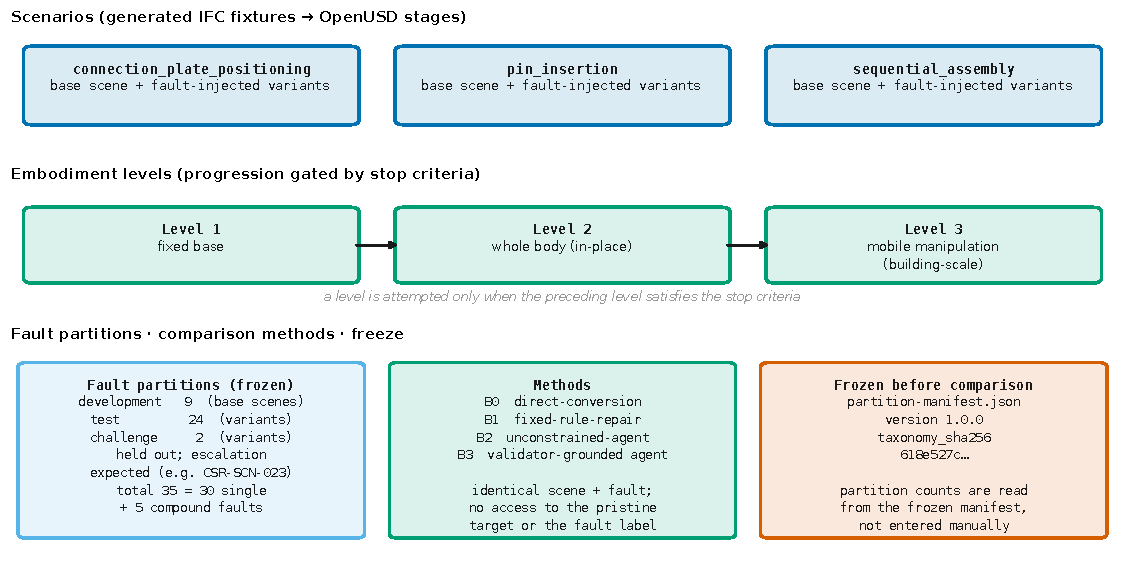
\includegraphics[width=\textwidth]{figures/fig06_benchmark.pdf}
\caption{Benchmark organization across construction scenarios, embodiment
levels, controlled scene defects, and comparison methods.}
\label{fig:benchmark-design}
\end{figure*}

\begin{table*}[t]
\centering
\caption{Planned benchmark composition. Counts marked TBD will be populated
from the frozen partition manifest rather than entered manually.}
\label{tab:benchmark}
\small
\resizebox{\textwidth}{!}{%
\begin{tabular}{p{0.19\textwidth}p{0.22\textwidth}p{0.18\textwidth}
p{0.14\textwidth}p{0.17\textwidth}}
\toprule
Scenario & Parameterization & Robot task levels & Faulted cases &
Primary outcome \\
\midrule
Connection-plate positioning & Component size, pose, target height,
work-zone obstacle & Fixed base; whole body; mobile & \placeholder{TBD after
split freeze} & Placement pose and state completion \\
Simplified pin insertion & Interface axis, clearance, friction, initial
misalignment & Fixed base; whole body; mobile & \placeholder{TBD after split
freeze} & Insertion depth without jam \\
Sequential assembly & Component order, temporary support, path obstruction,
state transition & Fixed base; whole body; mobile & \placeholder{TBD after
split freeze} & Complete legal task sequence \\
\bottomrule
\end{tabular}
}
\end{table*}

\subsection{Fault-injection benchmark}

Faults cover semantic identity, geometry and coordinates, physical properties,
assembly interfaces, construction states, and task references. Every injected
fault has a known location, severity, valid repair, and expected task
consequence. The current CPU suite comprises 30 single faults and five compound
faults. Development, test, and challenge partitions are frozen before the
agent comparison. The challenge partition includes faults that should be
rejected or escalated rather than repaired automatically. Consequential
findings are recorded separately from the injected root cause; for example, an
unresolved robot actor also prevents capability verification.

\subsection{Baselines and ablations}

The baselines are direct IFC geometry conversion, frozen deterministic
conversion with fixed repair, and unconstrained agentic repair. The full method
combines the scene contract, multi-scale compiler, deterministic validator,
provenance, and constrained agent selection from a whitelisted tool registry.
All methods receive the same scene and fault, and none may inspect the pristine
target scene or fault label during evaluation. Ablations remove provenance,
task-level validation, task-activated payloads, typed diagnostics, or agentic
tool selection one at a time.

\subsection{Metrics and statistical tests}

Static evaluation measures semantic preservation, relation F1, critical-fault
precision/recall/F1, repair success, incorrect repair, human escalation, and
runtime. Scene efficiency measures load time, peak memory, active prim count,
and collision-query cost. Task evaluation measures reachability,
collision-free planning, grasping, alignment, insertion, and complete-task
success.

Paired scenes are compared using McNemar tests for binary outcomes and
Wilcoxon signed-rank tests for time and iteration counts. Bootstrap confidence
intervals quantify uncertainty. Logistic regression tests whether readiness
scores predict task success while controlling for scenario and task level.
Language-model methods are repeated with at least five seeds per case, with
model version, decoding parameters, token use, and cost retained in the
experiment registry.

\begin{table*}[t]
\centering
\caption{Frozen comparison and ablation design. All methods receive identical
faulted scenes and are evaluated by the same post-repair validator and runtime
tasks.}
\label{tab:baselines}
\small
\resizebox{\textwidth}{!}{%
\begin{tabular}{p{0.19\textwidth}ccccc}
\toprule
Method & Construction IR & Multi-scale USD & Deterministic scene rules &
Provenance & Repair \\
\midrule
Direct conversion & -- & -- & -- & -- & -- \\
Fixed-rule conversion & -- & partial & -- & partial & fixed \\
Unconstrained agent & partial & partial & -- & partial & agent \\
Full method & \checkmark & \checkmark & \checkmark & \checkmark &
constrained agent \\
\bottomrule
\end{tabular}
}
\end{table*}
